\documentclass{beamer}

\mode<presentation>
 {\usetheme{CambridgeUS}
  \usecolortheme{beaver}
  \setbeamercovered{transparent}
  % appearance of bullets
  \useinnertheme{rectangles}
  \definecolor{mybullets}{rgb}{0.6,0.0,0.0}
  \setbeamercolor{structure}{fg=mybullets}

  \definecolor{mycolor}{rgb}{0.2,0.2,0.2}
  % bars
  %\setbeamercolor{section in toc}{fg=black,bg=white}
  %\setbeamercolor{alerted text}{fg=mycolor!80!gray}
  %\setbeamercolor*{palette primary}{fg=mycolor!60!black,bg=gray!30!white}
  %\setbeamercolor*{palette secondary}{fg=mycolor!70!black,bg=gray!15!white}
  %\setbeamercolor*{palette tertiary}{bg=mycolor!80!black,fg=gray!10!white}
  %\setbeamercolor*{palette quaternary}{fg=mycolor,bg=gray!5!white}
  %\setbeamercolor*{sidebar}{fg=mycolor,bg=gray!15!white}

  \setbeamercolor*{palette sidebar primary}{fg=mycolor!10!black}
  \setbeamercolor*{palette sidebar secondary}{fg=white}
  \setbeamercolor*{palette sidebar tertiary}{fg=mycolor!50!black}
  \setbeamercolor*{palette sidebar quaternary}{fg=gray!10!white}

  \setbeamercolor{titlelike}{parent=palette primary,fg=mycolor}
  \setbeamercolor{frametitle}{bg=gray!10!white}
  \setbeamercolor{frametitle right}{bg=gray!60!white}

  \setbeamercolor*{separation line}{}
  \setbeamercolor*{fine separation line}{}
}

 \def\Tiny{\fontsize{5pt}{5pt}\selectfont}
 \renewcommand{\arraystretch}{1.2}

% just show sections and subsections in table of contents
\setcounter{tocdepth}{2}

\usepackage[english]{babel}
\usepackage[latin1]{inputenc}

\usepackage{times}
\usepackage[T1]{fontenc}

\usepackage{hyperref}
\usepackage{multicol}

\newcommand{\todo}{\hspace{-2.3pt}$\bullet$ \hspace{5pt}}

\title[Profibus]{\textbf{Pro}cess \textbf{Fi}eld \textbf{Bus}}

\author[Koslowski]{Konstantin Koslowski (316955)}

\institute[]
{TU Berlin \\
 Department of Telecommunication Systems \\
 Telecommunication Networks Group \\
}

\date{June 19th, 2015}

\pgfdeclareimage[height=0.5cm]{university-logo}{tu-tkn-logo.jpg}
\logo{\pgfuseimage{university-logo}}

\begin{document}

\begin{frame}
  \titlepage
\end{frame}

\begin{frame}
\frametitle{Table of Contents}
\setcounter{tocdepth}{1}
\tableofcontents
\end{frame}

\section{Introduction}


\subsection{Development of Profibus}
\begin{frame}
\frametitle{Timeline}
  \textbf{1986}
  \begin{itemize}
    \item Master development plan ``fieldbus'' created in Germany
    \item 21 companies, including Siemens, involved
  \end{itemize}

  \textbf{1989}
  \begin{itemize}
    \item First promoted by \textit{Bundesministerium f\"ur Bildung und
        Forschung (BMBF)}
    \item Goal to implement a bit-serial field bus for factory and process automation
  \end{itemize}

  \textbf{1999}
  \begin{itemize}
    \item Published openly as part of standard \textbf{IEC 61158} \textit{Digital data
        communication for measurement and control - Fieldbus for use in industrial control
        systems}
  \end{itemize}
\end{frame}

\section{System Structure}
\begin{frame}
  \frametitle{System Structure: Introduction}
  \begin{itemize}
    \item \textit{Profibus} is a multi-master system
    \item Operation of multiple systems over a single bus
    \item Three protocols available
      \begin{itemize}
        \item FMS \textit{(field-bus message specification)}
        \item DP \textit{(decentralized peripheral)}
        \item PA \textit{(process automation)}
      \end{itemize}
    \item Devices are categorized in different types
      \begin{itemize}
        \item Masters
        \item Slaves
      \end{itemize}
  \end{itemize}
\end{frame}

\begin{frame}
  \frametitle{System Structure: Layer}
  \textit{Profibus} in the OSI reference model~\cite{profibusmanual}
  \center
  \footnotesize
  \begin{tabular}[h]{l|l|l}
    \textbf{Layer}  & \textbf{Name}     & \textbf{Content} \\
    \hline
    Layer 8         & User Layer        & Profiles \\
    Layer 7         & Application Layer & FMS / DP / PA protocol \\
    Layer 2         & Data Link Layer   & FDL protocol \\
    Layer 1         & Physical Layer    & Transmission Technology
  \end{tabular} \\
\end{frame}


\begin{frame}
  \frametitle{Device Type: Master}
  \begin{itemize}
    \item Active station
    \item Control the data traffic on the bus
    \item When having the \textit{bus access token}: \\
      send messages without external requests
  \end{itemize}
\end{frame}

\begin{frame}
  \frametitle{Device Type: Slave}
  \begin{itemize}
    \item Passive station
    \item No self-initiated bus access
    \item Immediate response to data requested by a master
    \item Can only be controlled by a single master
  \end{itemize}
\end{frame}

\section{Layer 1: Physical Layer}
\begin{frame}
  \frametitle{Physical Layer}
  \begin{itemize}
    \item \textit{Profibus FMS} and \textit{Profibus DP}
      \begin{itemize}
        \item Mostly using RS 485 transmission
        \item Optical transmission via FOC \textit{(fibre optical cable)} possible
      \end{itemize}
    \item \textit{Profibus PA}
      \begin{itemize}
        \item Uses MBP \textit{(Manchester bus powered)}, providing power supply
      \end{itemize}
  \end{itemize}
  \center
  \footnotesize
  \begin{tabular}[h]{l|l}
    \textbf{Type} & \textbf{Transmission technology} \\
    \hline
    0             & copper cable with RS 485 \\
    1             & synchronous MBP \\
    2             & synthetic FOC \\
    3             & glass FOC \\
    4             & HCS FOC
  \end{tabular} \\
  \hfill \\
  \normalsize
  Transmission technology (IRC 61784)~\cite{profibusmanual}
\end{frame}

\begin{frame}
  \frametitle{Physical Layer: RS 485}
  \begin{itemize}
    \item Bus-topology
    \item Twisted-pair cables with $150\Omega$
    \item Data rates from $9.6kbit/s$ to $12Mbit/s$
    \item Distance between repeaters $100m$ to $1200m$
    \item UART coding \\
      \footnotesize
      \begin{itemize}
        \item Start = 0, Parity = EVEN, Stop = 1 \\
        \item
          \begin{tabular}[h]{|c|c|c|c|c|c|c|c|c|c|c|}
            \hline
            Start & Databit 1 & 2 & 3 & 4 & 5 & 6 & 7 & 8 & Parity & Stop \\
            \hline
          \end{tabular}
      \end{itemize}
  \end{itemize}
  Mainly used with \textit{Profibus DP}
\end{frame}

\begin{frame}
  \frametitle{Physical Layer: FOC}
  \begin{itemize}
    \item Star-, bus or ring-topology
    \item Fibre optical cables
    \item Distance between repeaters up to $15km$
  \end{itemize}
\end{frame}

\begin{frame}
  \frametitle{Physical Layer: MBP}
  \begin{itemize}
    \item Bus-topology
    \item Stations are powered through the bus
    \item Safe in explosion-hazardous environments, power can be reduced to a bare minimum
    \item Data rate is fixed to $31.25kbit/s$
    \item Bus length up to $1900m$
    \item Allows branches up to $60m$ to field devices
    \item Manchester coding
  \end{itemize}
\end{frame}

\begin{frame}
  \frametitle{Physical Layer: MBP}
  Manchester coding \\
  \begin{itemize}
    \begin{multicols}{2}
    \item Every bit is coded as a change
      \begin{itemize}
        \item Positive change: ``0''
        \item Negative change: ``1''
        \item Every bit has the same average value
        \item Average used to power the peripherals
        \item Time synchronization possible with every bit
      \end{itemize}
      \columnbreak
      \begin{figure}[h]
        \centering
        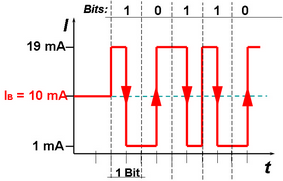
\includegraphics[width=140pt]{img/mbp}
        \caption{Manchester coding}
        \label{fig:mbp}
      \end{figure}
    \end{multicols}
  \end{itemize}
  Mainly used with \textit{Profibus PA}
\end{frame}

\section{Layer 2: Data Link Layer}
\begin{frame}
  \frametitle{Data Link Layer}
  The data transmission in \textit{Profibus} is handled by the \textit{fieldbus data link
    (FDL)} layer. \\
  FDL consists of three functions:
  \begin{itemize}
    \item Medium Access Control \textit{(MAC)}
    \item Fieldbus Link Control \textit{(FLC)}
    \item Fieldbus Management \textit{(FMA)}
  \end{itemize}
\end{frame}

\begin{frame}
  \frametitle{Data Link Layer: MAC}
  \begin{itemize}
    \item Make sure only one station transmits data on the bus
    \item When multiple masters are present
      \begin{itemize}
        \item Masters need the access token to send data
        \item Token is cyclically passed via token telegram
        \item To ensure that all master stations can access the bus, token must be passed
          on after a certain timeout
      \end{itemize}
    \item Slaves only respond to requests by a master
  \end{itemize}
  \textit{Profibus FDL} combines master-slave and token passing in a hybrid access principle
\end{frame}

\begin{frame}
  \frametitle{Data Link Layer: FMA}
  Fieldbus Management provides functions to manage the layer 1 and 2
    \begin{itemize}
      \item Reset the layers
      \item Set parameters
      \item Get parameters
      \item Inform the user about events or errors
      \item Activate/Deactivate \textit{service access point (SAP)}
    \end{itemize}
\end{frame}

\begin{frame}
  \frametitle{Data Link Layer: Error handling}
  Errors can be caused by
  \begin{itemize}
    \item Faulty transmitters
    \item Badly shielded cables
    \item Signal reflections
    \item Large divergences in time synchronization between stations
  \end{itemize}
  Error rate is smaller than $10^{-4}$ and can be reduced further by error detection and
  correction
\end{frame}

\begin{frame}
  \frametitle{Data Link Layer: Error detection and correction}
  Error Detection
  \begin{itemize}
    \item Hamming distance of 4 by adding a checksum to each packet
    \item At least 4 bits must change to result in an undetected error
    \item This results in \textit{integrity class 2} after standard \textbf{IEC 870-5-1}
  \end{itemize}

  \vspace{10pt}
  \textit{Send Data with No acknowledge (SDN)} service
  \begin{itemize}
    \item Mainly used for synchronization and status messages
    \item The erroneous telegram is discarded
    \item Telegram from the next cycle is used instead
  \end{itemize}
\end{frame}

\begin{frame}
  \frametitle{Data Link Layer: Error detection and correction}
  \textit{Send Data with Acknowledge (SDA)}
  \begin{itemize}
    \item Mainly used between masters, slaves may not always send an acknowledgement
    \item When the sender does not get a response, the telegram is retransmitted
  \end{itemize}

  \vspace{10pt}
  \textit{Send and Request Data (SRD)}
  \begin{itemize}
    \item Service used between masters and slaves
    \item Acknowledgement is packed on top of the data telegram
    \item When the sender does not get a response, the telegram is retransmitted
  \end{itemize}
\end{frame}


\section{Layer 7: Application Layer}
\begin{frame}
  \frametitle{Application Layer: Addressing}
  \begin{itemize}
    \item Every station has a unique address, coded in 1 byte
      \center
      \footnotesize
      \begin{tabular}[h]{l|l}
        \textbf{Address}  & \textbf{Use} \\
        \hline
        $0$               & reserved for tools, e.g.\ programming devices \\
        $1 - n$           & $n$ master stations \\
        $n - 125$         & slave stations \\
        $126$             & reserved as \textit{delivery address} \\
                          & used for changing the address of a slave during runtime \\
        $127$             & reserved as broadcast address
      \end{tabular}
  \end{itemize}
  Components used for the infrastructure, e.g.\ repeaters transmit the data transparently
  and do not require an address \\
\end{frame}

\begin{frame}
  \frametitle{Application Layer: Telegram Formats}
  \begin{itemize}
    \item Without data field \\
      % \footnotesize
      % \begin{tabular}[h]{|c|c|c|c|c|c|}
      %   \hline
      %   SD1 & DA & SA & FC & FCS & ED \\
      %   \hline
      % \end{tabular}
      % \vspace{5pt}
      % \tiny
      % SD1: Delimiter, DA: Destination Address, SA: Source Address, \\
      % FC: Function Code, FCS: Frame Check Sequence, ED: End Delimiter
      % \normalsize
    \item Variable length from $4-249$ byte, payload $1-246$ byte \\
      \footnotesize
      \begin{tabular}[h]{|c|c|c|c|c|c|c|c|c|c|}
        \hline
        SD2 & LE & LEr & SD2 & DA & SA & FC & PDU & FCS & ED \\
        \hline
      \end{tabular} \\
      \vspace{3pt}
      \tiny
      SD2: Delimiter, LE: Length, LEr: Length repeated, DA: Destination Address,
      SA: Source Address, FC: Function Code, \\
      \vspace{-5pt}
      PDU: Protocol Data Unit, FCS: Frame Check Sequence, ED: End Delimiter
      \normalsize
    \item Fixed payload length of $8$ bytes
      % \footnotesize
      % \begin{tabular}[h]{|c|c|c|c|c|c|c|}
      %   \hline
      %   SD3 & DA & SA & FC & PDU & FCS & ED \\
      %   \hline
      % \end{tabular}
      % \normalsize
    \item Token telegram
      % \footnotesize
      % \begin{tabular}[h]{|c|c|c|}
      %   \hline
      %   SD4 & DA & SA \\
      %   \hline
      % \end{tabular}
      % \normalsize
    \item Short telegram
      % \footnotesize
      % \begin{tabular}[h]{|c|}
      %   \hline
      %   SDC \\
      %   \hline
      % \end{tabular}
      % \normalsize
      \hfill \\
    \item Telegram Delimiter, featuring a Hamming distance of 4 \\
      \footnotesize
      \begin{tabular}[h]{|c|c|c|c|c|c|}
        \hline
        SD1   & SD2   & SD3   & SD4   & ED    & SC \\
        \hline
        0x10  & 0x68  & 0xA2  & 0xDC  & 0x16  & 0xE5 \\
        \hline
      \end{tabular}
      \normalsize
  \end{itemize}
\end{frame}

\begin{frame}
  \frametitle{Application Layer: FMS}
  \begin{itemize}
    \item FMS master controls the relationship with FMS slaves
    \item Replaced by \textit{Profibus DP}
  \end{itemize}
\end{frame}

\begin{frame}
  \frametitle{Application Layer: DP}
  \begin{itemize}
    \item \textit{Profibus DP} masters are separated into classes
      \begin{itemize}
        \item Class 1: control a DP system and the slaves assigned, mostly PLC based
        \item Class 2: tool for commissioning, engineering and maintenance, mostly PC
          based
        \item Class 3: clock master, used for time synchronization
      \end{itemize}
      \center
      \begin{figure}
        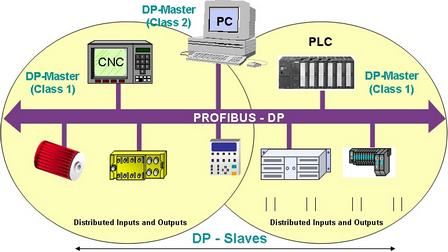
\includegraphics[width=.50\textwidth]{img/dp_system.png}
        \caption{Structure of a DP system~\cite{profibusmanual}}
      \end{figure}
  \end{itemize}
\end{frame}

\begin{frame}
  \frametitle{Application Layer: DP - Cyclic process data}
  Data exchange between masters and slaves is separated into three
  phases:~\cite{profibusmanual}
  \center
  \footnotesize
  \begin{tabular}[h]{l|l}
    \textbf{Phase}  & \textbf{Action} \\
    \hline
    Diagnosis       & Master requests diagnostic data from slaves \\
    Initialization  & Master sets parameters and checks configuration of slaves \\
    Data Exchange   & Master sends and requests data from the slaves
  \end{tabular} \\
\end{frame}

\begin{frame}
  \frametitle{Application Layer: DP - Data Exchange}
  Class 1 master station:
  \begin{itemize}
    \item Relationship with a slave is called \textit{MS0}
    \item Data exchange is cyclic
    \item Master sends output data to a slave
    \item Slave immediately responds with input data
    \item Master continues with the next slave or restarts the cycle
  \end{itemize}
  \vspace{10pt}
  The minimum cycle time $T_{BCycle}$ can be calculated:
  \begin{align}
    T_{BCycle} = \frac{380 + (N_{Slaves} \cdot 300) + (N_{Bytes} \cdot 11)}{Bitrate} + 75
    \mu s
    \label{minimumcycletime}
  \end{align}
\end{frame}

\begin{frame}
  \frametitle{Application Layer: DP - Data Exchange}
  Class 2 master station:
  \begin{itemize}
    \item Can exist in addition class 1 masters
    \item Can simultaneously be a class 1 master
    \item Relationship with a slave is called \textit{MS1}
    \item Acyclic communication with a slave in an existing MS0 relationship
  \end{itemize}
\end{frame}

\begin{frame}
  \frametitle{Application Layer: PA}
  \begin{itemize}
    \item Uses the same protocol as \textit{Profibus DP}
    \item Can be connected to an existing \textit{Profibus DP} network
      \begin{itemize}
        \item Using a DP/PA coupler
        \item The faster \textit{DP} network is used as a backbone
      \end{itemize}
  \end{itemize}
\end{frame}

\section*{References}
\begin{frame}[allowframebreaks]
  \frametitle{References}
  \begin{thebibliography}{10}
  \beamertemplatebookbibitems
  \bibitem{profibusmanual}
    Max Felser
    \newblock Profibus Manual: A collection of information explaining PROFIBUS networks
    \newblock http://www.profibus.felser.ch

    \bibitem{profibuswiki}
    Wikipedia
    \newblock Profibus
    \newblock https://en.wikipedia.org/wiki/Profibus

    \bibitem{fieldbuswiki}
    Wikipedia
    \newblock Fieldbus
    \newblock https://en.wikipedia.org/wiki/Fieldbus
   \end{thebibliography}
 \end{frame}
\end{document}
